\documentclass[a4paper,12pt]{article}
\usepackage[utf8]{inputenc}
\usepackage[MeX]{polski}
\usepackage{fixltx2e}
\usepackage[table,xcdraw]{xcolor}
\usepackage[utf8]{inputenc}
\usepackage[T1]{fontenc}
\usepackage{graphicx}
\usepackage{color}
\usepackage{mathtools}
%%%%%%%%%%%%%%%%%%%%%%%%%%%%%%%%%%%%%%%%%%%%%%%%%%%%%%%%%%%%%STRONA TYTULOWA%%%%%%%%%%%%%%%%%%%%%%%%%%%%%%%%%%%%%%%%%%%%%%%%%%%%%%%%%%%%%%%%%%%%%%%%
\title{\Huge \textbf{Politechnika Wrocławska\\[0.3in]} 
  \huge Katedra Teorii Pola, Układów elektronicznych i Optoelektronicznych \\[0.2in]
  \LARGE Zespół Układów Elektronicznych
}
\date{}
\author{}

\begin{document}
\maketitle

\begin{table}[h]
  \large
  \centering
  \begin{tabular}{|ll|l|}
    \hline
    \multicolumn{1}{|l|}{Data: 14.04.2015r}                  & \multicolumn{2}{l|}{Dzień: Wtorek}                                     \\ \hline
    \multicolumn{1}{|l|}{Grupa: VII}                        & \multicolumn{2}{l|}{Godzina: 12:15-15:00}                               \\ \hline
    \multicolumn{3}{|l|}{\textit{\begin{tabular}[c]{@{}l@{}}\textbf{Temat ćwiczenia:} \\ Przetwornice DC/DC\end{tabular}}}		 \\ \hline
    \textbf{Dane projektowe:}                               & \multicolumn{2}{l|}{}                                             	 \\
    \multicolumn{1}{|l}{    U\textsubscript{we}=9.00 V }   & \multicolumn{1}{l}{R\textsubscript{SC}=0.625\Omega}&  \multicolumn{1}{l|}{L=330uH} \\ 
    \multicolumn{1}{|l}{    U\textsubscript{wy}=6.00 V }   & \multicolumn{1}{l}{R\textsubscript{1}=1.795\Omega}&  \multicolumn{1}{l|}{C\textsubscript{0}=476uF} \\ 
    \multicolumn{1}{|l}{    I\textsubscript{max}=9.00 V }  & \multicolumn{1}{l}{R\textsubscript{2}=6.720k\Omega}&  \multicolumn{1}{l|}{C\textsubscript{T}=560pF} \\ \hline
    \multicolumn{1}{|l|}{\textbf{l.p}}                    & \textbf{Nazwisko i imię}                 & \textbf{Oceny}               \\ \hline
    \multicolumn{1}{|l|}{1}                               & Arkadiusz Ziółkowski                     &                               \\ \hline
    \multicolumn{1}{|l|}{2}                               & Jakub Koban                              &                                \\ \hline
  \end{tabular}
\end{table}


%%%%%%%%%%%%%%%%%%%%%%%%%%%%%%%%%%%%%%%%%%%%%%%%%%%%%%%%%%%%%%%%%%%%%%%%%%%%%%%%%%%%%%%%%%%%%%%%%%%%%%%%%%%%%%%%%%%%%%%%%%%%%%%%%%%%%%%%%%%%%%%%%%%%
%%%%%%%%%%%%%%%%%%%%%%%%%%%%%%%%%%%%%%%%%%%%%%%%%%%%%%%%%%%%%%%%%%%ZADANIE PROJEKTOWE%%%%%%%%%%%%%%%%%%%%%%%%%%%%%%%%%%%%%%%%%%%%%%%%%%%%%%%%%%%%%%%
%%%%%%%%%%%%%%%%%%%%%%%%%%%%%%%%%%%%%%%%%%%%%%%%%%%%%%%%%%%%%%%%%%%%%%%%%%%%%%%%%%%%%%%%%%%%%%%%%%%%%%%%%%%%%%%%%%%%%%%%%%%%%%%%%%%%%%%%%%%%%%%%%%%%
\pagebreak
\section{Zadanie projektowe}
Zaprojektować zasilacz stabilizowany obniżający napięcie o zadanych parametrach:
\begin{itemize}
\item U\textsubscript{we}=9.00 V
\item U\textsubscript{wy}=6.00 V
\item I\textsubscript{max}=0.25 A
\end{itemize}
%%%%%%%%%%%%%%%%%%%%%%%%%%%%%%%%%%%%%%%%%%%%%%%%%%%%%%%%%%%%%%%%%%%%%%%%%%%%%%%%%%%%%%%%%%%%%%%%%%%%%%%%%%%%%%%%%%%%%%%%%%%%%%%%%%%%%%%%%%%%%%%%%%%%
%%%%%%%%%%%%%%%%%%%%%%%%%%%%%%%%%%%%%%%%%%%%%%%%%%%%%%%%%%%%%%%%%%%CZĘŚĆ PROJEKTOWA%%%%%%%%%%%%%%%%%%%%%%%%%%%%%%%%%%%%%%%%%%%%%%%%%%%%%%%%%%%%%%%%%
%%%%%%%%%%%%%%%%%%%%%%%%%%%%%%%%%%%%%%%%%%%%%%%%%%%%%%%%%%%%%%%%%%%%%%%%%%%%%%%%%%%%%%%%%%%%%%%%%%%%%%%%%%%%%%%%%%%%%%%%%%%%%%%%%%%%%%%%%%%%%%%%%%%%
\section{Obliczenia projektowe}

\begin{equation}
I_{pk}=I_{Lpk}=2I_{max}=2*0.25=0.5 A
\end{equation}

\begin{equation}
\mathbf{R_{SC}}=\frac{0.3V}{I_{pk}}=\frac{0.3}{0.5}=\mathbf{0.6 \Omega}
\end{equation}

\begin{equation}
Zakładamy \quad \mathbf{R_1=1.8k\Omega}   \quad \to \quad   \mathbf{R_2}=R_1 \frac {|U_{wy}|-1.25V}{1.25V} = 1800\frac{6-1.25}{1.25}= \mathbf{6.8k \Omega}
\end{equation}

\begin{equation}
Zakładamy \quad \mathbf{T=25u}s \quad \to \quad \mathbf{t_{on}}=T\frac{U_0}{U_i}=25*10^{-6}\frac{6}{9}=\mathbf{16.67us}
\end{equation}

\begin{equation}
\mathbf{L}\geq\frac{U_i}{I_{Lpk}}t_{ON}=\frac{9}{0.5}*16.37*10^{-6}=\mathbf{300uH}
\end{equation}

\begin{equation}
\mathbf{C_0}\geq\frac{I_{Lpk}T}{8U_{tpp}}=\frac{0.5*25*10^{-6}}{8*0.5}=\mathbf{3.125uF}
\end{equation}
\newpage
%%%%%%%%%%%%%%%%%%%%%%%%%%%%%%%%%%%%%%%%%%%%%%%%%%%%%%%%%%%%%%%%%%%%%%%%%%%%%%%%%%%%%%%%%%%%%%%%%%%%%%%%%%%%%%%%%%%%%%%%%%%%%%%%%%%%%%%%%%%%%%%%%%%%
\section {Schemat projektowy}
\begin{figure}[h]
  \center
  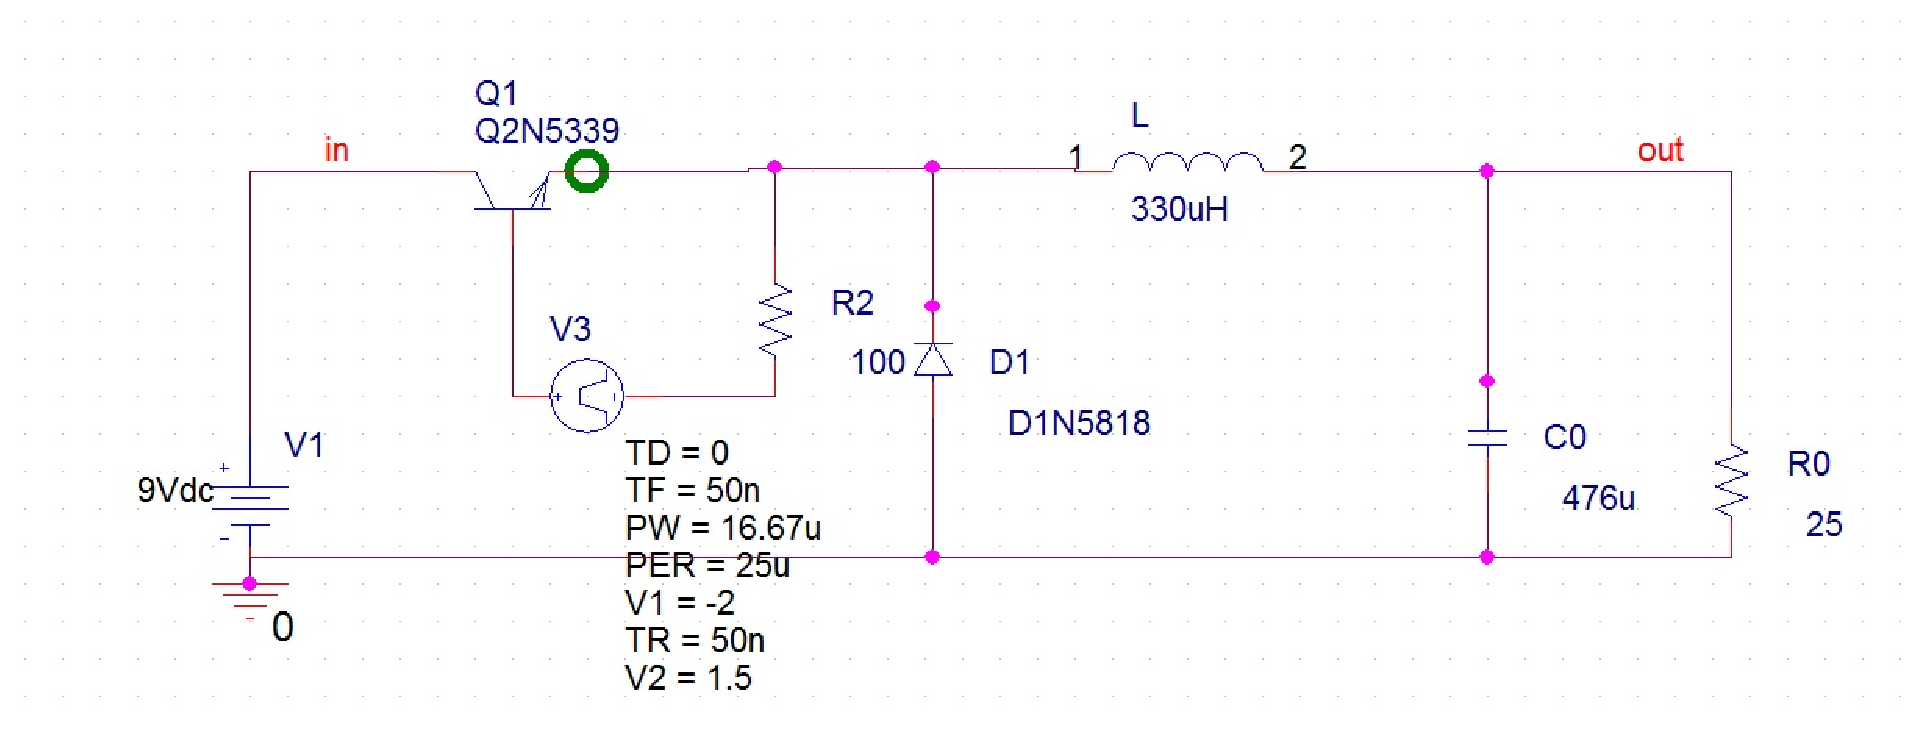
\includegraphics[width=0.7\textwidth]{schemat_sim.eps}
  \caption{Schemat do symulacji projektowanego układu}

  \center
  \includegraphics[width=0.3\textwidth]{wyk.eps}
  \caption{Symulacja --------- obrazek do porawienia}

  \center
  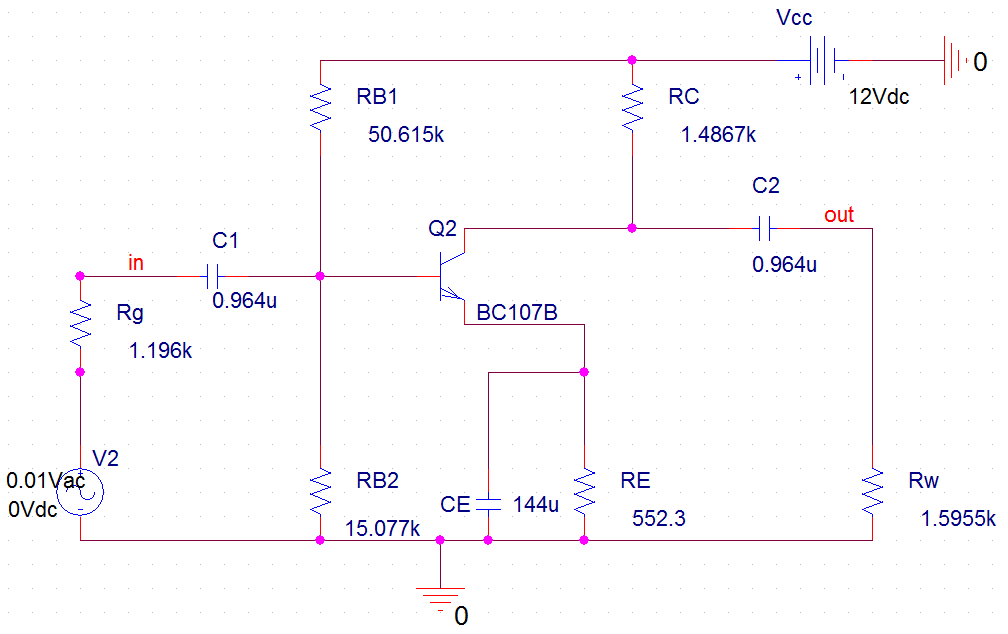
\includegraphics[width=0.7\textwidth]{schemat.eps}
  \caption{Schemat projektowanego układu}
\end{figure}

\pagebreak
%%%%%%%%%%%%%%%%%%%%%%%%%%%%%%%%%%%%%%%%%%%%%%%%%%%%%%%%%%%%%%%%%%%%%%%%%%%%%%%%%%%%%%%%%%%%%%%%%%%%%%%%%%%%%%%%%%%%%%%%%%%%%%%%%%%%%%%%%%%%%%%%%%%%
%%%%%%%%%%%%%%%%%%%%%%%%%%%%%%%%%%%%%%%%%%%%%%%%%%%%%%%%%%%%%%%%%%%CZĘŚĆ LABORATORYJNA%%%%%%%%%%%%%%%%%%%%%%%%%%%%%%%%%%%%%%%%%%%%%%%%%%%%%%%%%%%%%%
%%%%%%%%%%%%%%%%%%%%%%%%%%%%%%%%%%%%%%%%%%%%%%%%%%%%%%%%%%%%%%%%%%%%%%%%%%%%%%%%%%%%%%%%%%%%%%%%%%%%%%%%%%%%%%%%%%%%%%%%%%%%%%%%%%%%%%%%%%%%%%%%%%%%
\section{Część laboratoryjna}
\subsection{Charakterystyka napięciowa i napięciowo - prądowa}
%\begin{table}[ht]
  \begin{center}
  \begin{tabular}{|r|r|r|r|r|r|r|r|}
    \hline
    \multicolumn{2}{|c|}{\textbf{Stałe obciążenie}} &  & \multicolumn{5}{c|}{\textbf{Zmienne obciążenie}} \\ \cline{1-2} \cline{4-8}
    \textbf{$U_{we}[V]$} & \textbf{$U_{wy}[V]$} & & \textbf{$U_{we}[V]$} & \textbf{$I_{we}[mA]$} & \textbf{$U_{wy}[V]$} & \textbf{$I_{wy}[mA]$} &\textbf{$\eta $ } \\ \cline{1-2} \cline{4-8}
    0		& 0	&	& 9	& 25.82		& 6.197		& 27.91		& 0.74  \\ \cline{1-2} \cline{4-8}
    0.5		& 0.001 &	& 9 	& 36.87		& 6.192		& 41.32		& 0.77 \\ \cline{1-2} \cline{4-8}
    0.9		& 0.010	&	& 9	& 44.92		& 6.191		& 51.02		& 0.78	\\ \cline{1-2} \cline{4-8}
    1.5		& 0.200	&	& 9 	& 66.82		& 6.188		& 77.11		& 0.79 \\ \cline{1-2} \cline{4-8}
    2.0		& 0.586	&	& 9	& 93.56		& 6.184		& 108.47	& 0.80 \\ \cline{1-2} \cline{4-8}
    2.5		& 0.940 &	& 9	& 134.13	& 6.178		& 154.98	& 0.79 \\ \cline{1-2} \cline{4-8}
    3.0		& 1.340 &	& 9	& 168.09	& 6.126		& 195.13	& 0.79 \\ \cline{1-2} \cline{4-8}
    3.5		& 1.750 &	& 9	& 228.10	& 5.840		& 269.77	& 0.77 \\ \cline{1-2} \cline{4-8}
    4.0		& 2.170	&	& 9	& 269.00	& 5.518		& 330.00	& 0.75 \\ \cline{1-2} \cline{4-8}
    4.5		& 2.570	&	& 9	& 300.50	& 4.791		& 408.50	& 0.72 \\ \cline{1-2} \cline{4-8}
    5.0		& 3.040 &	& 9	& 270.70	& 3.808		& 445.30 	& 0.70 \\ \cline{1-2} \cline{4-8}
    5.5		& 3.480 &	& 9	& 250.80	& 3.331		& 464.80 	& 0.69 \\ \cline{1-2} \cline{4-8}
    6.0		& 3.860	&	& \multicolumn{5}{c|}{} \\ \cline{1-2} 
    6.5		& 4.320	&	& \multicolumn{5}{c|}{} \\ \cline{1-2} 
    7.0		& 4.670	&	& \multicolumn{5}{c|}{} \\ \cline{1-2} 
    7.5		& 5.120 &	& \multicolumn{5}{c|}{} \\ \cline{1-2} 
    8.0		& 5.500	&	& \multicolumn{5}{c|}{} \\ \cline{1-2} 
    8.5		& 6.140	&	& \multicolumn{5}{c|}{} \\ \cline{1-2} 
    9.0		& 6.180 &	& \multicolumn{5}{c|}{} \\ \cline{1-2} 
    9.5		& 6.180	&	& \multicolumn{5}{c|}{} \\ \cline{1-2} 
    10.0	& 6.190 &	& \multicolumn{5}{c|}{} \\ \cline{1-2} 
    10.5	& 6.190	&	& \multicolumn{5}{c|}{} \\ \cline{1-2} 
    11.0	& 6.192 &	& \multicolumn{5}{c|}{} \\ \cline{1-2} 
    11.5	& 6.192 &	& \multicolumn{5}{c|}{} \\ \cline{1-2} 
    12.0	& 6.194 &	& \multicolumn{5}{c|}{} \\ \cline{1-2} 
    12.5	& 6.194 &	& \multicolumn{5}{c|}{} \\ \cline{1-2} 
    13.0	& 6.196 &	& \multicolumn{5}{c|}{} \\ \cline{1-2} 
    13.5	& 6.196 &	& \multicolumn{5}{c|}{} \\ \cline{1-2} 
    14.0	& 6.199 &	& \multicolumn{5}{c|}{} \\ \cline{1-2} 
    14.5	& 6.208 &	& \multicolumn{5}{c|}{} \\ \cline{1-2} 
    15.0	& 6.206 &	& \multicolumn{5}{c|}{} \\ \hline
  \end{tabular}
  \end{center}
  
%\end{table}
%\pagebreak
%%%%%%%%%%%%%%%%%%%%%%%%%%%%%%%%%%%%%%%%%%%%%%%%%%%%%%%%%%%%%%%%%%%%%%%%%%%%%%%%%%%%%%%%%%%%%%%%%%%%%%%%%%%%%%%%%%%%%%%%%%%%%%%%%%%%%%%%%%%%%%%%%%%%

\begin{figure}[h!]
  \begin{center}
  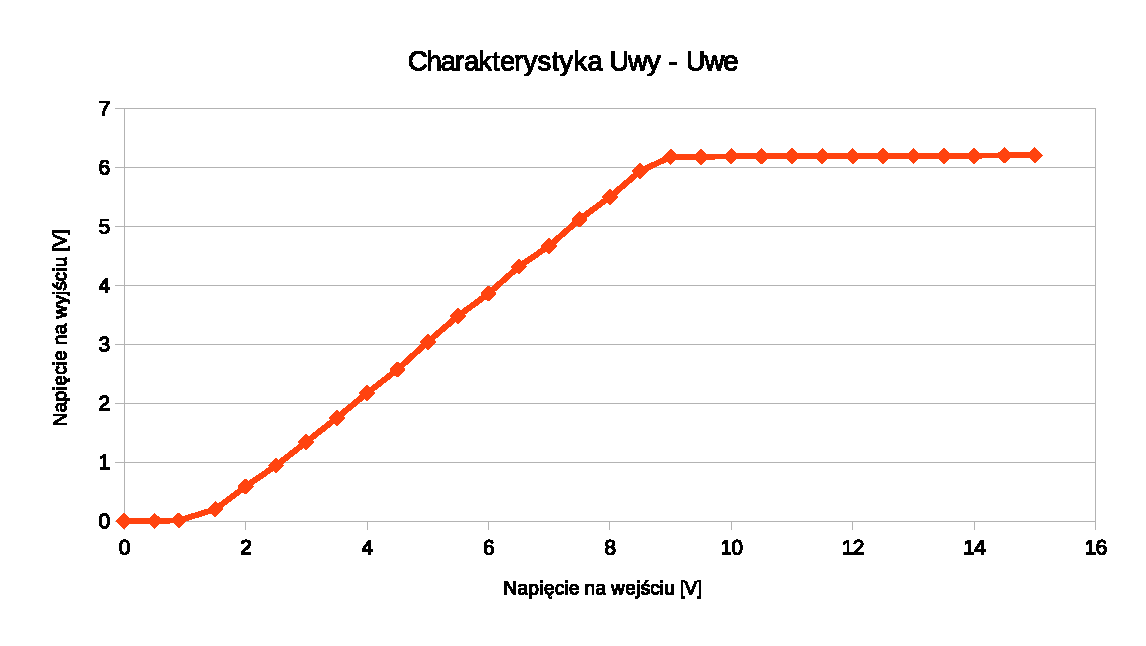
\includegraphics[width=0.85\textwidth]{Uwe_Uwy.eps}
  \caption{Charakterystyka napięcia wyjściowego od napięcia wejściowego przy stałym obciążeniu}
  \end{center}

Na powyższjej charakterystyce widzimy, że zasilacz poprawnie stabilizuje napięcie wyjściowe na zadanym poziomie
dla napięcia wejściowego mieszczącego się w przedziale od 8.5V do 15V.

  \begin{center}
  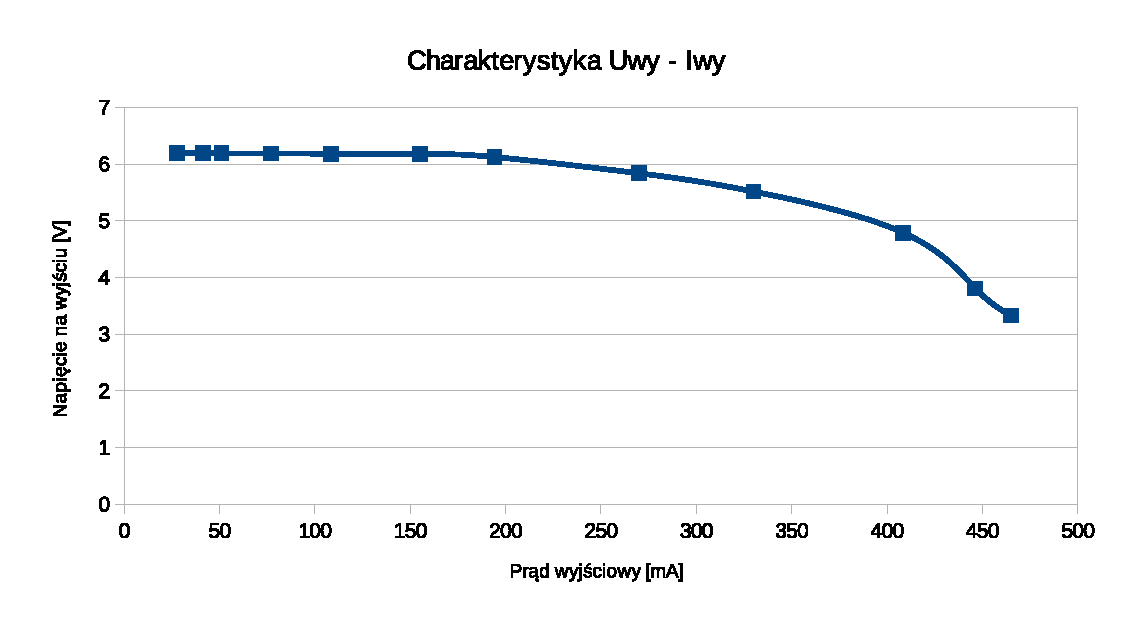
\includegraphics[width=0.85\textwidth]{Uwy_Iwy.eps}
  \caption{Charakterystyka natężenia prądu wyjściowego od napięcia wyjściowego przy zmiennym obciążeniu}
  \end{center}

Z powyższego wykresu widzimy, iż przy natężeniu prądu wyjściowego przekraczającemu wartość ok 225 mA 
napięcie na wyjściu zasilacza spada poniżej 6V.
\end{figure}

\pagebreak

\begin{figure}[h!]
  \begin{center}
  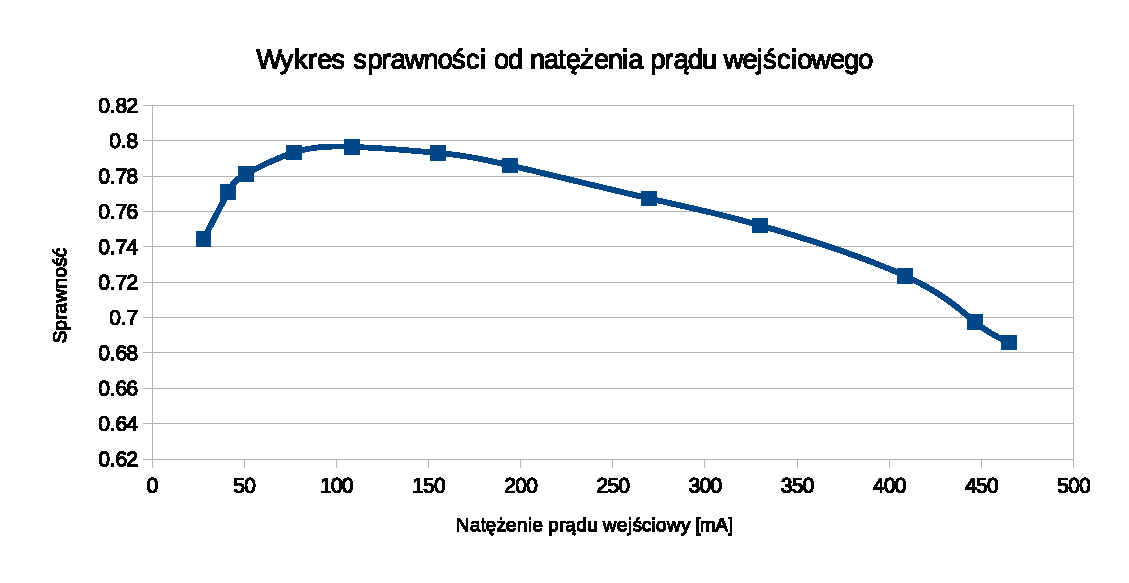
\includegraphics[width=0.85\textwidth]{spr_Iwy.eps}
  \caption{Wykres sprawności od natężenia prądu wyjściowego}
  \end{center}
  
  Tutaj możemy zauważyć, że sprawność zasilacza w warunkach pracy tj. dla natężenia prądu wyjściowego w zakresie od
kilkudziesięciu mili amperów do około 250mA utrzymuje się na poziomie powyżej 0.74, gdzie maksimum osiąga 
dla ok. 100mA natężenia prądu wyjściowego i wynosi około 0.79.
Warto też dodać, iż dla niskich natężeń prądu wyjściowego zmiany sprawności są bardzo szybkie.
\end{figure}

%%%%%%%%%%%%%%%%%%%%%%%%%%%%%%%%%%%%%%%%%%%%%%%%%%%%%%%%%%%%%%%%%%%%%%%%%%%%%%%%%%%%%%%%%%%%%%%%%%%%%%%%%%%%%%%%%%%%%%%%%%%%%%%%%%%%%%%%%%%%%%%%%%%%

%%%%%%%%%%%%%%%%%%%%%%%%%%%%%%%%%%%%%%%%%%%%%%%%%%%%%%%%%%%%%%%%%%%%%%%%%%%%%%%%%%%%%%%%%%%%%%%%%%%%%%%%%%%%%%%%%%%%%%%%%%%%%%%%%%%%%%%%%%%%%%%%%%%%

\section {Wnioski}

\begin{itemize}
  \item Na podstawie Rysunku nr 4 widzimy, iż zasilacz pracuje zgodnie z oczekiwaniami teoretycznymi, ponieważ dla 
	napięcia nominalnego $U_{we} = 9V$ na wyjściu otrzymujemy zadane napięcie ok. 6V.
  \item Wykres z rysunku nr 5 wskazuje na to, że układ został zaprojektowany i wykonany zgodnie z założeniami
	projektowymi, gdyż dla wartości od kilkudziesięciu mA do ok. 225mA natężenia prądu wyjściowego 
	układ utrzymuje zadane napięcie wyjściowe na poziomie ok. 6V. Zakres ten jest o ok. 25mA mniejszy
	od założonego $I_{max} = 250mA$. Wynika to najprawdopodobniej z użycia nieco innych wartości
	elementów niż zakłdają obliczenia projektowe.
  \item Sprawność wyrysowana w zależności od natężenia prądu wyjściowego na rystunku nr 6 przyjmuje 
	wartości na poziomie 0.7 - 0.8 co możemy uznać za wartości mieszczące się w normach tego typu układów.
\end{itemize}

\end{document}
